\documentclass{article}

\usepackage{amsmath,amssymb}
\usepackage{geometry}
\usepackage{graphicx}

\geometry{a4paper, margin=2.5cm}

\begin{document}

% ============================================================
\section*{Deep Q-Networks (DQN)}

\subsection*{First, a story}

In 2013, DeepMind published a paper doing something that sounded crazy: with one codebase and one set of hyperparameters, let an AI play Atari games. Nobody told it the rules --- only screen pixels and the score, like a kid with no manual mashing buttons in front of the TV.

By 2015, the upgraded version beat most of 49 games, matching or exceeding human level on Breakout, Pong and others. This AI is \textbf{DQN (Deep Q-Network)}.

Before DQN, a recognized chasm separated deep neural networks from reinforcement learning: \textbf{training instability}. Approximating $Q$ with a network often diverged. DQN closed it with two elegant engineering tricks.

\textbf{The core question of this chapter}: Q-learning already works --- why does it need DQN?

% ============================================================
\section*{Why a Q Table Is Not Enough --- the Curse of Dimensionality}

Recall the Q-learning update:
\[
Q(s,a) \leftarrow Q(s,a) + \alpha\!\left[r + \gamma \max_{a'} Q(s',a') - Q(s,a)\right]
\]

The algorithm needs a \textbf{Q table}: one number per state--action pair $(s,a)$. In a discrete grid world that is fine. In CartPole the state is 4 continuous numbers (cart position, velocity, pole angle, angular velocity) --- the table would have infinitely many rows.

Discretizing does not save you:

\[
\begin{array}{c|c}
\text{Bins per dimension} & \text{CartPole Q-table entries (4 dims, 2 actions)} \\
\hline
b = 10  & 10^4 \times 2 = 20{,}000 \\
b = 20  & 20^4 \times 2 = 320{,}000 \\
b = 100 & 100^4 \times 2 = 200{,}000{,}000 \\
\end{array}
\]

An Atari state is an $84 \times 84 \times 4$ stack of grayscale frames --- about $256^{84\times 84\times 4}$ table entries, beyond writing down (Figure~\ref{fig:qtable}).

\begin{figure}[!htbp]
  \centering
  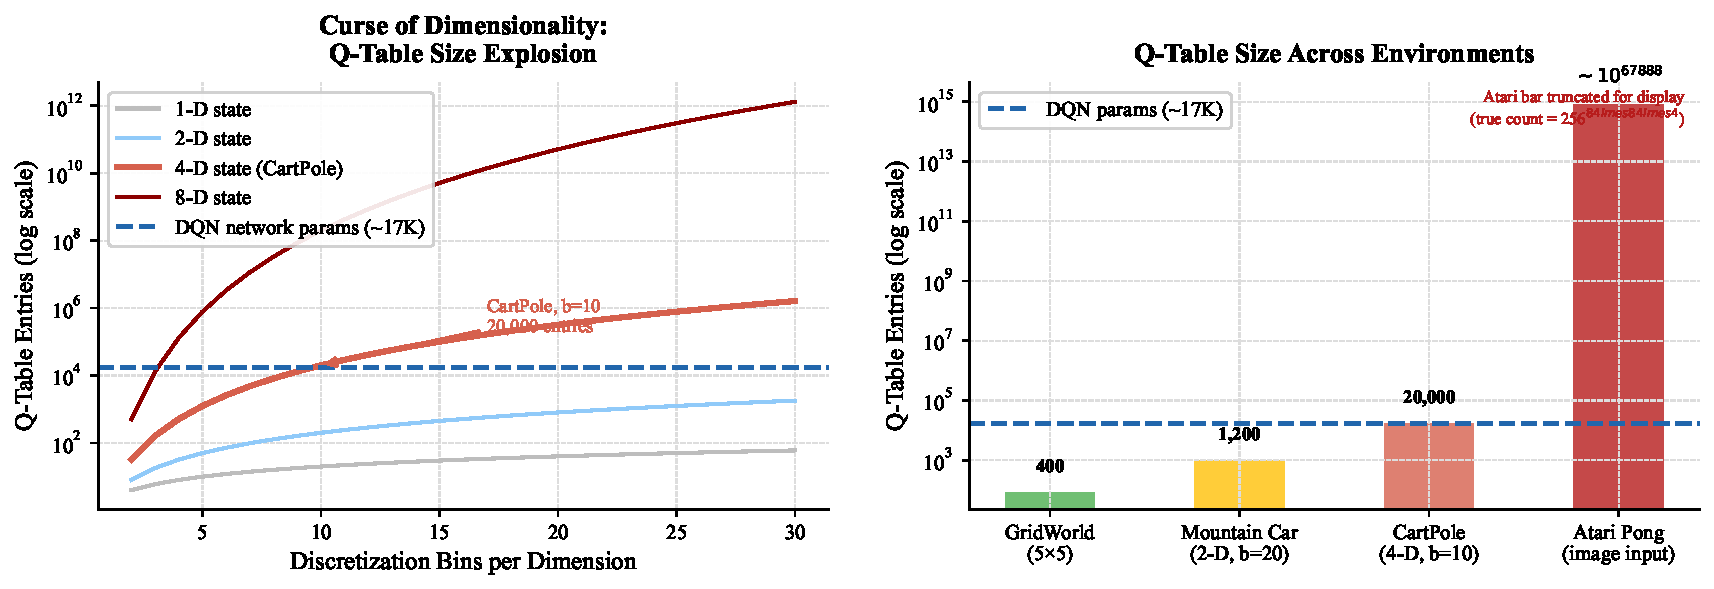
\includegraphics[width=0.95\textwidth]{fig1_qtable_motivation.pdf}
  \caption{The curse of dimensionality: Q-table size explodes exponentially with state dimension and discretization resolution, far beyond the parameter count of a small neural network.}
  \label{fig:qtable}
\end{figure}

\textbf{The way out}: stop storing a table; fit $Q(s,a)$ with a \textbf{function}.

% ============================================================
\section*{Innovation 1: Approximating $Q$ with a Neural Network}

\subsection*{From Q table to Q network}

Replace the table by a network with parameters $\theta$:
\[
\boxed{Q(s, a;\, \theta) \approx Q^*(s, a)}
\]

The input is the state $s$; the output is \textbf{the vector of Q values for all actions} --- one forward pass yields every action's estimate:
\[
a^* = \arg\max_{a}\, Q(s, a;\, \theta)
\]

\subsection*{The loss}

Training pulls predictions toward Bellman targets with a squared loss:
\[
\boxed{\mathcal{L}(\theta) = \mathbb{E}_{(s,a,r,s') \sim \mathcal{D}}\!\left[\Bigl(r + \gamma \max_{a'} Q(s', a';\, \theta^-) - Q(s, a;\, \theta)\Bigr)^2\right]}
\]

Here $\mathcal{D}$ is the experience dataset and $\theta^-$ the target-network parameters (detailed below).

\subsection*{Two fatal problems of naive training}

Naively descending on each transition $(s, a, r, s')$ hits:
\begin{itemize}
  \item \textbf{Problem 1 --- temporal correlation}: consecutive frames are nearly identical; gradient estimates have high variance and training oscillates;
  \item \textbf{Problem 2 --- the moving target}: the target $r + \gamma\max_{a'}Q(s',a';\theta)$ itself moves with $\theta$ --- chasing a moving target, Q values easily diverge.
\end{itemize}

DQN's other two innovations each address one of these precisely.

% ============================================================
\section*{Innovation 2: Experience Replay}

\subsection*{The problem: temporal correlation}

Online Q-learning updates the network after every step. Adjacent states are highly correlated (cart leaning right $\to$ next frame still leaning right), violating the i.i.d.\ assumption behind stochastic gradient descent: gradient variance blows up and training oscillates.

\subsection*{The fix: a replay buffer}

Store every transition $(s, a, r, s', \mathrm{done})$ in a FIFO \textbf{replay buffer} $\mathcal{D}$ (capacity $N$); at training time sample a mini-batch \textbf{uniformly at random}:

\[
\boxed{\{(s_i, a_i, r_i, s_i')\}_{i=1}^{B} \;\sim\; \mathrm{Uniform}(\mathcal{D})}
\]

\subsection*{Why it works}

\begin{itemize}
  \item \textbf{Breaks temporal correlation}: random sampling makes batches approximately i.i.d., restoring the SGD assumption;
  \item \textbf{Improves data efficiency}: each experience can be sampled many times;
  \item \textbf{Stabilizes gradients}: larger batch $B$ means lower gradient variance.
\end{itemize}

The ablation in Figure~\ref{fig:replay} shows it: without replay, training curves have much larger variance and slower convergence.

\begin{figure}[!htbp]
  \centering
  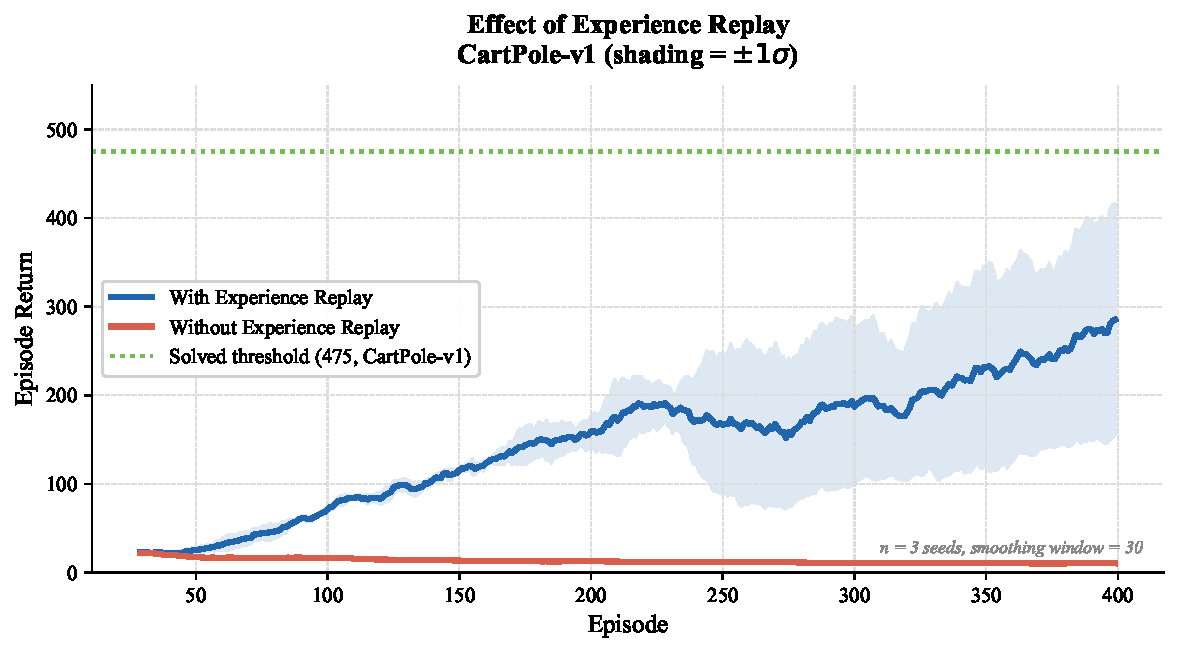
\includegraphics[width=0.88\textwidth]{fig2_replay_comparison.pdf}
  \caption{Experience-replay ablation (CartPole-v1, 3 random seeds, shading $\pm 1\sigma$). With replay the run converges faster with less variance.}
  \label{fig:replay}
\end{figure}

% ============================================================
\section*{Innovation 3: The Target Network}

\subsection*{The problem: the moving target}

In naive DQN both sides of the loss contain $\theta$:
\[
\mathcal{L}(\theta) = \mathbb{E}\!\left[\Bigl(\underbrace{r + \gamma \max_{a'} Q(s', a';\, \theta)}_{\text{target}} - \underbrace{Q(s, a;\, \theta)}_{\text{prediction}}\Bigr)^2\right]
\]

Every gradient step moves the prediction toward the target --- but the target moves with $\theta$ too. This is \textbf{chasing a moving target}: updating one Q value indirectly drags others, triggering cascading instability until the values diverge.

\subsection*{The fix: a frozen target network}

Maintain two networks:
\begin{itemize}
  \item \textbf{Online network} $Q(s,a;\theta)$: updated by gradient descent every step, used to choose actions;
  \item \textbf{Target network} $Q(s,a;\theta^-)$: \textbf{frozen}; it only enters Bellman targets and is hard-synced from the online network every $C$ steps:
\end{itemize}
\[
\boxed{\theta^- \;\leftarrow\; \theta \quad \text{(every } C \text{ steps; frozen in between)}}
\]

The loss becomes:
\[
\mathcal{L}(\theta) = \mathbb{E}\!\left[\Bigl(\underbrace{r + \gamma \max_{a'} Q(s', a';\, \theta^-)}_{\text{fixed target (short-term)}} - Q(s, a;\, \theta)\Bigr)^2\right]
\]

\textbf{Intuition}: swap ``a target that moves every step'' for ``one that shifts every $C$ steps'' --- over the short term the target is static and training is far more stable. Larger $C$ means a steadier but more stale $\theta^-$; the value is task-dependent --- the Atari paper used $C=10^4$, small tasks typically $10^2 \sim 10^3$.

The ablation is shown in Figure~\ref{fig:target}.

\begin{figure}[!htbp]
  \centering
  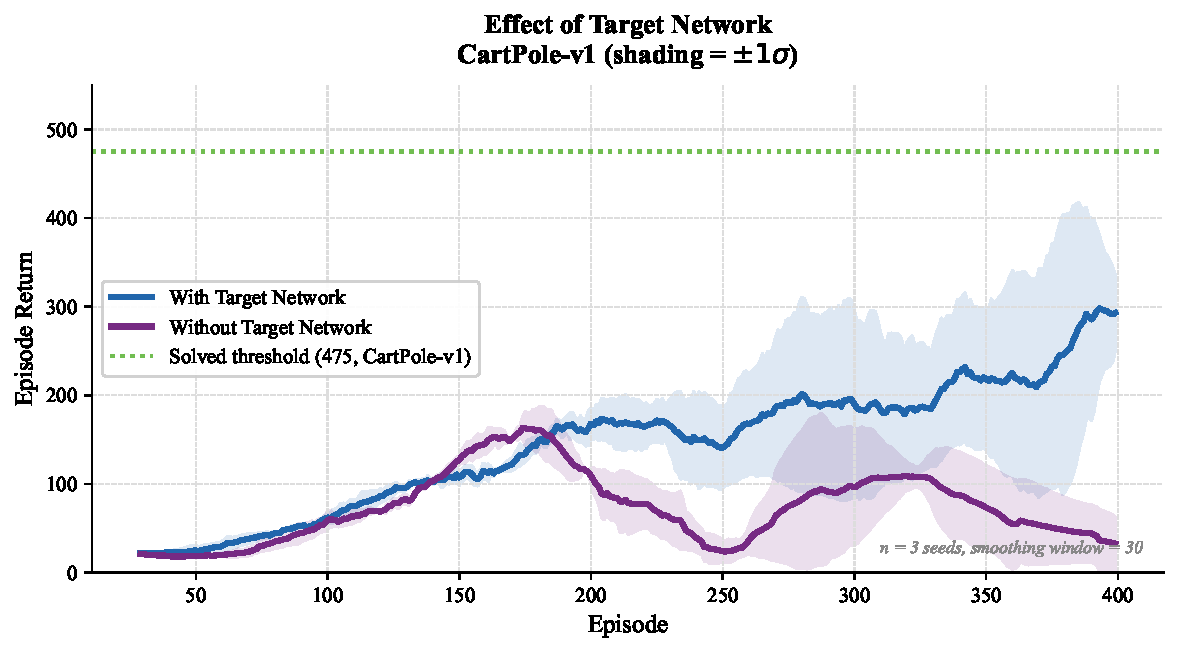
\includegraphics[width=0.88\textwidth]{fig3_target_comparison.pdf}
  \caption{Target-network ablation (CartPole-v1, 3 random seeds, shading $\pm 1\sigma$). Without a target network the training curve is less stable with higher variance across seeds.}
  \label{fig:target}
\end{figure}

% ============================================================
\section*{The Full DQN Algorithm}

Combining the three innovations:

\begin{enumerate}
  \item \textbf{Initialize}: replay buffer $\mathcal{D}$ (capacity $N$), online parameters $\theta$, target $\theta^- \leftarrow \theta$, exploration rate $\varepsilon$;
  \item \textbf{Each episode}, for each step $t$:
  \begin{enumerate}
    \item choose $\varepsilon$-greedily:
          \[a_t = \begin{cases} \text{random} & \text{with probability } \varepsilon \\ \arg\max_{a} Q(s_t, a;\theta) & \text{with probability } 1-\varepsilon \end{cases}\]
    \item execute $a_t$, observe $r_t$, $s_{t+1}$; store $(s_t, a_t, r_t, s_{t+1}, \mathrm{done})$ in $\mathcal{D}$;
    \item sample $B$ transitions uniformly; compute Bellman targets:
          \[y_i = \begin{cases} r_i & \text{if terminal} \\ r_i + \gamma \max_{a'} Q(s_i', a';\theta^-) & \text{otherwise} \end{cases}\]
    \item gradient step: $\displaystyle\theta \leftarrow \theta - \alpha \nabla_\theta \frac{1}{B}\sum_{i=1}^B \bigl(y_i - Q(s_i, a_i;\theta)\bigr)^2$;
    \item every $C$ steps: $\theta^- \leftarrow \theta$.
  \end{enumerate}
\end{enumerate}

\textbf{The three innovations in one line each}:

\begin{center}
\small
\begin{tabular}{l|l|l}
\textbf{Problem} & \textbf{Innovation} & \textbf{Operation} \\
\hline
unbounded state space & network approximation & $Q(s,a;\theta) \approx Q^*(s,a)$ \\[4pt]
temporally correlated samples & experience replay & $(s,a,r,s') \sim \mathrm{Uniform}(\mathcal{D})$ \\[4pt]
unstable targets & target network & $\theta^- \leftarrow \theta$ every $C$ steps\\
\end{tabular}
\end{center}

% ============================================================
\section*{Where DQN sits in the RL landscape}

DQN is the starting point of deep RL, inheriting classic RL and opening the deep-RL mainline:

\begin{enumerate}
  \item \textbf{From tables to networks}: Q-learning (tabular, small discrete states) $\to$ DQN (network, continuous high-dimensional states); the update rule is identical, only the approximator changed;
  \item \textbf{Replay's long shadow}: a fixed dataset plus offline learning is precisely the paradigm of \textbf{offline RL} --- the data of later algorithms such as CQL and IQL all comes from some form of replay buffer;
  \item \textbf{Evolution of the target network}: hard update $\theta^- \leftarrow \theta$ $\to$ soft (Polyak) update $\theta^- \leftarrow (1-\tau)\theta^- + \tau\theta$, adopted widely by DDPG, TD3 and SAC;
  \item \textbf{Next steps}: Double DQN (decoupling action selection from evaluation to curb overestimation) and Dueling DQN (splitting $Q$ into $V$ plus advantage $A$) --- both precise upgrades within the DQN framework.
\end{enumerate}

\subsection*{References}

\begin{enumerate}
  \item Mnih, V., et al.\ (2013). Playing Atari with Deep Reinforcement Learning. \textit{NeurIPS Deep Learning Workshop}.
  \item Mnih, V., et al.\ (2015). Human-level control through deep reinforcement learning. \textit{Nature}, 518, 529--533.
  \item Sutton, R.\,S.\ \& Barto, A.\,G.\ (2018). \textit{Reinforcement Learning: An Introduction} (2nd ed.). Chapters 9--10.
  \item Hands-on RL (Chinese). Chapter 7: the DQN algorithm.
\end{enumerate}

\end{document}
